\documentclass{article}
\usepackage{graphicx} % Required for inserting images
\usepackage{float}

\title{Foundations of Data Science Final Project}
\author{Asif M. Abdul Hameed}
\date{October 2026}

\begin{document}

\maketitle

\section{Introduction}

Breast cancer is a heterogeneous disease with substantial variation in
molecular characteristics and gene expression across tumors. The Cancer
Genome Atlas Breast Invasive Carcinoma (TCGA-BRCA) project provides
genomic and clinical data that can be used to investigate these molecular
differences in breast cancer \cite{TCGA2012}. In this project, RNA
sequencing (RNA-seq) gene expression count data and corresponding
clinical and molecular metadata from the TCGA-BRCA cohort were analyzed.

ERBB2 was selected as the primary gene of interest for this analysis.
ERBB2 encodes human epidermal growth factor receptor 2 (HER2), a receptor
tyrosine kinase with an important role in the development and treatment
of breast cancer. Increased HER2 expression is characteristic of a
clinically important subset of breast cancers and has led to the
development of multiple HER2-targeted therapies \cite{Gutierrez2011}.

My clinical interest in ERBB2 is also related to my work in pulmonary
medicine. HER2-targeted antibody-drug conjugates, including trastuzumab
deruxtecan, are associated with interstitial lung disease (ILD) and
drug-induced pneumonitis \cite{Tarantino2021}. As a pulmonologist with
a clinical focus on ILD, I encounter pulmonary toxicities associated
with cancer therapies in clinical practice. This connection between
ERBB2-targeted therapy and lung toxicity provided additional motivation
for selecting ERBB2 as the primary gene for this analysis.

\section{Methods}

RNA-seq gene expression count data and corresponding clinical and
molecular metadata from the TCGA-BRCA cohort were analyzed
\cite{GDCBRCA} using R version 4.6.1. Data manipulation and summary statistics were performed using tidyverse version 2.0.0, including dplyr version
1.2.1. Data visualizations were generated using ggplot2 version
4.0.3. ComplexHeatmap version 2.28.0 and circlize version 0.4.18
were used to generate the gene expression heatmap.

The RNA-seq count matrix contained gene-level expression counts, with
genes represented by Ensembl identifiers and samples represented by
TCGA sample identifiers. ERBB2 was selected as the primary gene of
interest, and descriptive statistics including the mean, median,
standard deviation, minimum, and maximum were calculated for ERBB2
expression. CDK4 was selected as a second gene for comparison with
ERBB2. Gene expression data were combined with the corresponding
clinical and molecular metadata using TCGA sample identifiers.
PAM50 molecular subtype was selected as the primary categorical
covariate, and age at initial pathologic diagnosis was selected as
an additional clinical covariate.

A histogram was used to examine the distribution of ERBB2 expression,
with the mean and median indicated by reference lines. A scatter plot
was used to compare ERBB2 and CDK4 expression, with a linear regression
line added to visualize their relationship. Because the RNA-seq counts
were right-skewed and spanned a wide range of values, log10 scales were
used for the gene expression axes. ERBB2 expression across PAM50
molecular subtypes was examined using a violin plot with an overlaid
box plot and a cumulative distribution function (CDF). Finally, a
heatmap was generated using a panel of 10 breast cancer-related genes.
For the heatmap, raw counts were transformed using log2(count + 1),
and both genes and samples were hierarchically clustered. PAM50
molecular subtype was included as a sample annotation.

\section{Results}

\subsection{Clinical and Molecular Characteristics}

Table 1 summarizes the distribution of PAM50 molecular subtypes and
age at initial pathologic diagnosis in the TCGA-BRCA cohort. Among
samples with available PAM50 classification, Luminal A was the most
common subtype (52.0\%), followed by Luminal B (19.0\%), Basal
(17.9\%), HER2-enriched (7.5\%), and Normal-like (3.6\%). The mean
age at initial pathologic diagnosis was 58.42 years.

\begin{table}[H]
\centering
\caption{Summary of selected clinical and molecular covariates}
\begin{tabular}{lll}
\hline
Covariate & Statistic & Value \\
\hline
PAM50 subtype & Basal, n (\%) & 197 (17.9\%) \\
 & HER2-enriched, n (\%) & 82 (7.5\%) \\
 & Luminal A, n (\%) & 571 (52.0\%) \\
 & Luminal B, n (\%) & 209 (19.0\%) \\
 & Normal-like, n (\%) & 40 (3.6\%) \\
\hline
Age at initial pathologic diagnosis & Mean & 58.42 years \\
 & Median & 58 years \\
 & Standard deviation & 13.15 years \\
 & Minimum & 26 years \\
 & Maximum & 90 years \\
\hline
\end{tabular}
\end{table}

\subsection{Distribution of ERBB2 Expression}

ERBB2 RNA-seq counts demonstrated a right-skewed distribution, with a
mean of 46,982.49 counts and a median of 19,125 counts. The standard
deviation was 105,287.5 counts, with values ranging from 205 to 995,067
counts. The mean exceeded the median due to a subset of samples with
substantially higher expression. A log10 scale was used to better
visualize the distribution across the wide range of ERBB2 expression
counts (Figure~\ref{fig:erbb2_histogram}).

\begin{figure}[H]
    \centering
    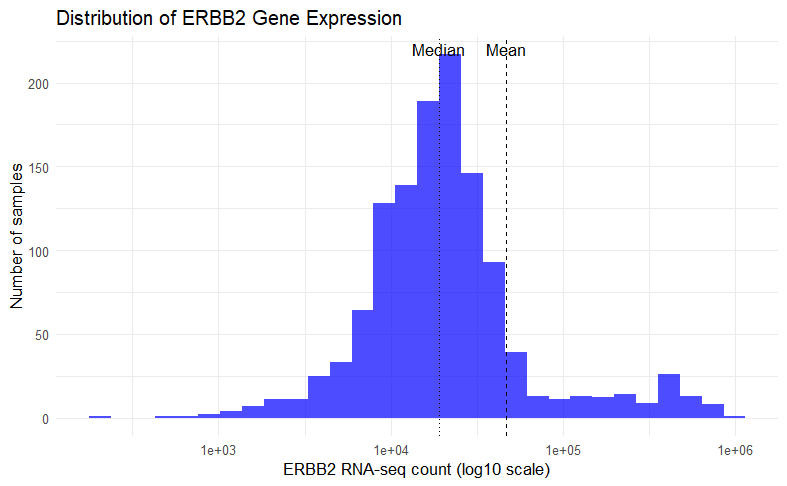
\includegraphics[width=0.8\textwidth]{ERBB2_histogram.png}
    \caption{Distribution of ERBB2 RNA-seq counts in the TCGA-BRCA
    cohort. The x-axis is displayed on a log10 scale. The dashed and
    dotted vertical lines represent the mean and median, respectively.}
    \label{fig:erbb2_histogram}
\end{figure}

\subsection{Relationship Between ERBB2 and CDK4 Expression}

ERBB2 and CDK4 expression demonstrated a modest positive relationship,
although substantial variability was present across samples. Log10
scales were used for both axes because of the wide range of RNA-seq
counts. A fitted linear regression line was included to visualize the
overall relationship between the two genes
(Figure~\ref{fig:erbb2_cdk4}).

\begin{figure}[H]
    \centering
    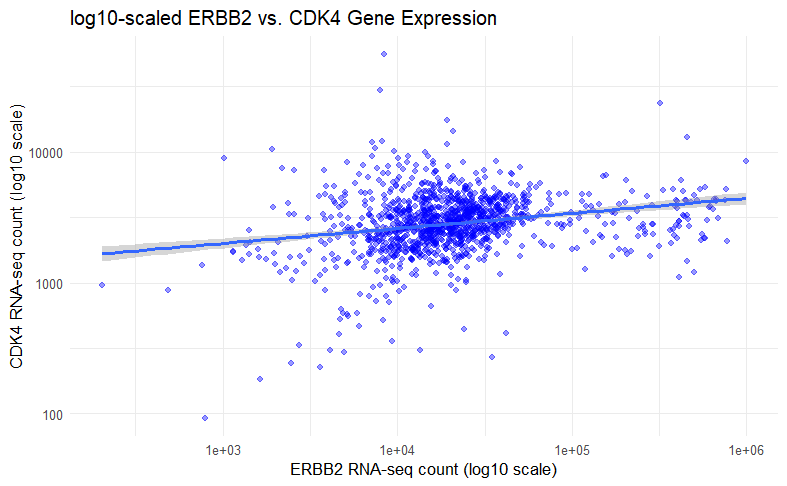
\includegraphics[width=0.8\textwidth]{ERBB2_CDK4_scatter.png}
    \caption{Relationship between ERBB2 and CDK4 RNA-seq counts in the
    TCGA-BRCA cohort. Both axes are displayed on log10 scales, and the
    fitted line represents a linear regression trend.}
    \label{fig:erbb2_cdk4}
\end{figure}

\subsection{ERBB2 Expression Across PAM50 Molecular Subtypes}

ERBB2 expression differed across PAM50 molecular subtypes. The
HER2-enriched subtype demonstrated substantially higher ERBB2 expression
overall, although considerable variability was present within the
subtypes. The violin plot displays the distribution of ERBB2 expression,
while the overlaid box plots show the median and interquartile range
(Figure~\ref{fig:erbb2_pam50_violin}).

\begin{figure}[H]
    \centering
    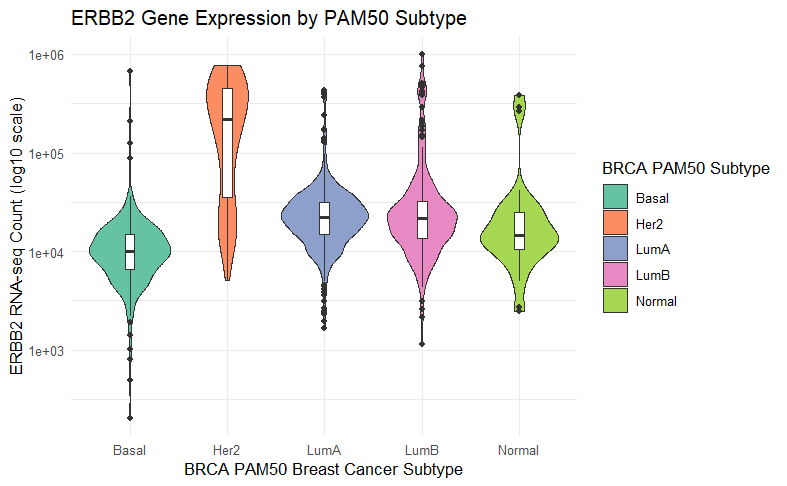
\includegraphics[width=0.8\textwidth]{ERBB2_PAM50_violin.png}
    \caption{Distribution of ERBB2 RNA-seq counts across PAM50 molecular
    subtypes in the TCGA-BRCA cohort. ERBB2 expression is displayed on
    a log10 scale. Violin plots represent the distribution of expression,
    and the overlaid box plots display the median and interquartile range.}
    \label{fig:erbb2_pam50_violin}
\end{figure}

\subsection{Cumulative Distribution of ERBB2 Expression}

The cumulative distribution of ERBB2 expression further demonstrated
differences among PAM50 molecular subtypes. The HER2-enriched subtype
showed a rightward shift in the distribution, indicating generally
higher ERBB2 expression compared with the other subtypes. Basal tumors
generally demonstrated lower ERBB2 expression, while the remaining
subtypes showed intermediate distributions
(Figure~\ref{fig:erbb2_pam50_cdf}).

\begin{figure}[H]
    \centering
    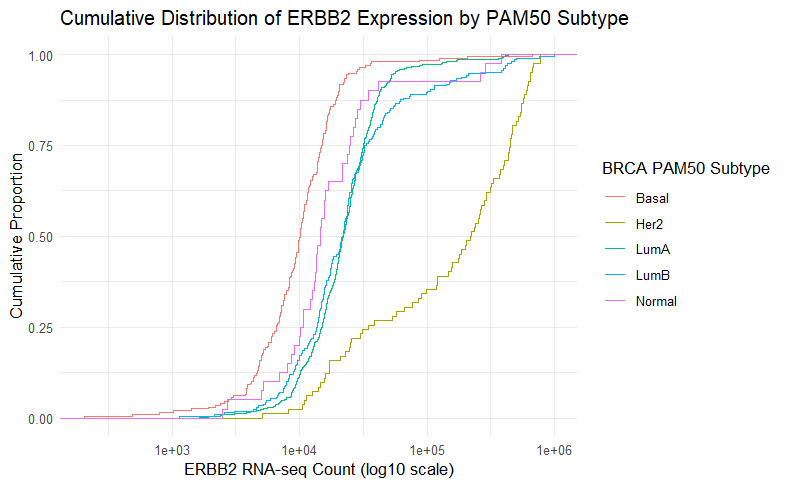
\includegraphics[width=0.8\textwidth]{ERBB2_PAM50_CDF.png}
    \caption{Cumulative distribution of ERBB2 RNA-seq counts across
    PAM50 molecular subtypes in the TCGA-BRCA cohort. ERBB2 expression
    is displayed on a log10 scale.}
    \label{fig:erbb2_pam50_cdf}
\end{figure}

\subsection{Gene Expression Heatmap}

The heatmap demonstrated distinct patterns of gene expression across
the TCGA-BRCA samples and PAM50 molecular subtypes. ERBB2 expression
was higher in many samples classified as HER2-enriched. Other
subtype-associated patterns were also visible, including lower ESR1
and PGR expression and higher KRT5 and EGFR expression in many
Basal samples. Hierarchical clustering grouped samples and genes
according to similarities in their expression patterns
(Figure~\ref{fig:heatmap}).

\begin{figure}[H]
    \centering
    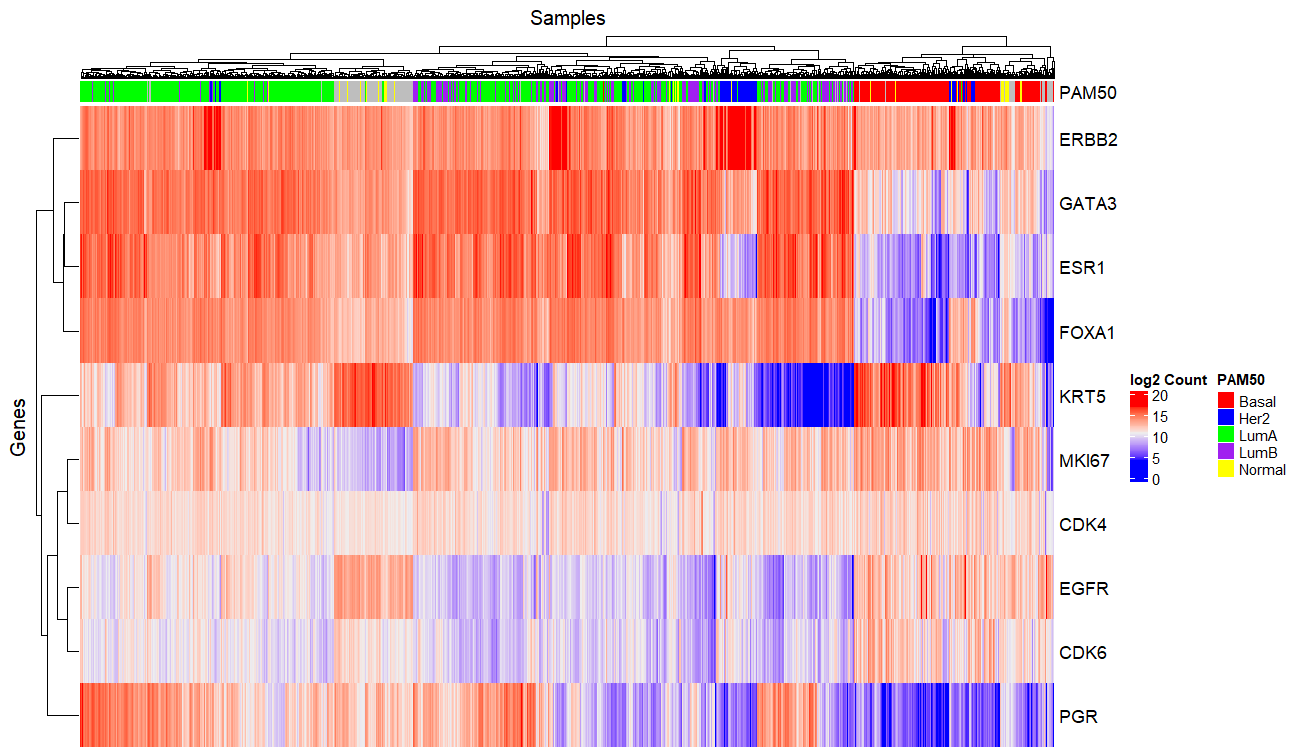
\includegraphics[width=0.95\textwidth]{Breast_Cancer_Heatmap.png}
    \caption{Heatmap of 10 breast cancer-related genes across TCGA-BRCA
    samples. RNA-seq counts were transformed using log2(count + 1).
    Rows represent genes and columns represent samples. Hierarchical
    clustering was performed for both genes and samples, and PAM50
    molecular subtype is shown as the sample annotation.}
    \label{fig:heatmap}
\end{figure}




\section*{Acknowledgments}

ChatGPT (OpenAI) was used to assist with reviewing and correcting R code
and with drafting and formatting portions of this report. The analyses,
interpretation of results, and final content were reviewed and verified
by the author.

\begin{thebibliography}{9}

\bibitem{TCGA2012}
The Cancer Genome Atlas Network. (2012).
Comprehensive molecular portraits of human breast tumours.
\textit{Nature, 490}(7418), 61--70.
doi:10.1038/nature11412.

\bibitem{Gutierrez2011}
Gutierrez, C., \& Schiff, R. (2011).
HER2: Biology, detection, and clinical implications.
\textit{Archives of Pathology \& Laboratory Medicine, 135}(1), 55--62.
doi:10.5858/2010-0454-RAR.1.

\bibitem{Tarantino2021}
Tarantino, P., Modi, S., Tolaney, S. M., Cortés, J., Hamilton, E. P.,
Kim, S.-B., Toi, M., Andrè, F., \& Curigliano, G. (2021).
Interstitial lung disease induced by anti-ERBB2 antibody-drug conjugates:
A review.
\textit{JAMA Oncology, 7}(12), 1873--1881.
doi:10.1001/jamaoncol.2021.3595.

\bibitem{GDCBRCA}
National Cancer Institute. (2026).
TCGA Breast Invasive Carcinoma (TCGA-BRCA).
\textit{Genomic Data Commons Data Portal}.
Accessed October 2026.

\end{thebibliography}

\end{document}
